\section{Spielfeld}
    In dem folgenden Kapitel wird das Spielfeld, dessen Aufbau in Zellen und die interne Repräsentation, 
    als Buffer, im Speicher erläutert.


    \subsection{Zelle}
        Eine Zelle wird auf dem LCD als Block von Pixeln wiedergegeben.
        Dabei besteht die Zelle aus folgender Formel:
        \begin{align}
        64 Pixel = 8 Pixel \cdot 8 Pixel
        \end{align}
        Diese 64 Pixel werden intern als acht hintereinander liegende Bytes repräsentiert.
        Dabei steht das erste Bit des ersten Bytes für den Pixel in der oberen linke Ecke.
        Um ein Pixel anzusteuern, wird das jeweilige Bit auf \textit{1} bzw. auf \textit{0} gesetzt.
        \begin{figure}[H]
            \centering
            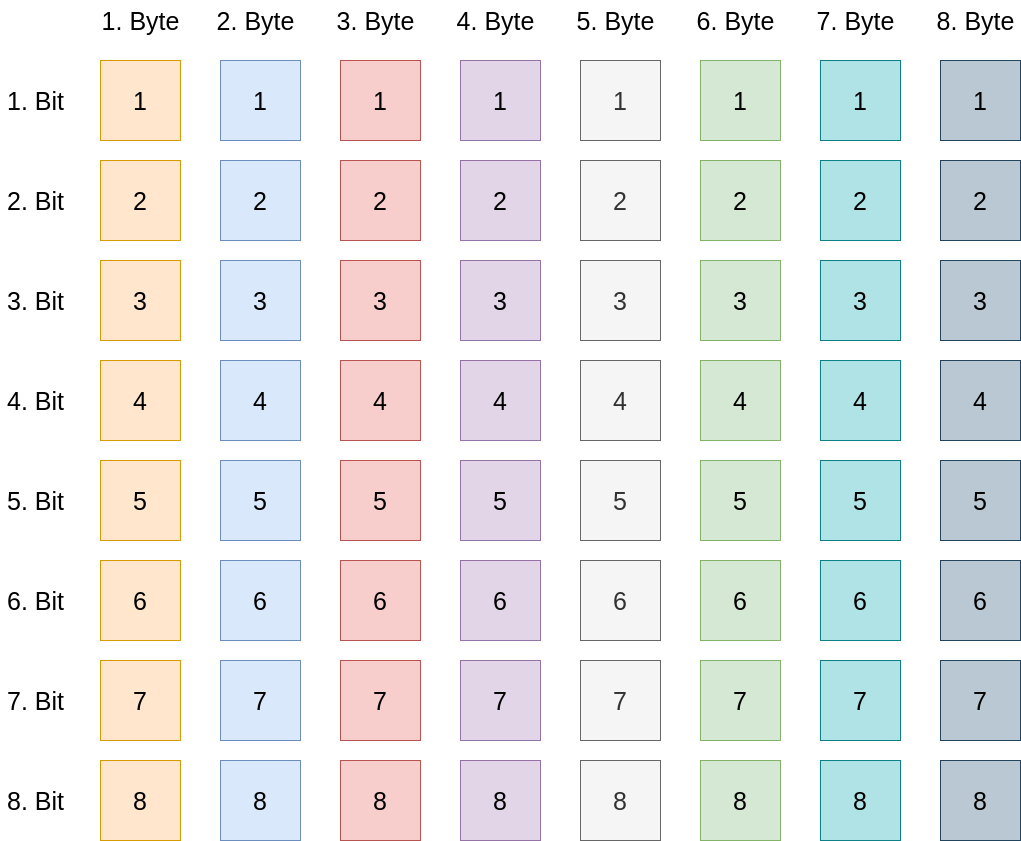
\includegraphics[scale=0.25]{img/zelle.png}    
            \caption{Darstellung einer Zelle im RAM}
        \end{figure}
    
    \subsubsection{Leere Zelle}
        Eine Leere Zelle ist jene, die kein Spielstein beinhaltet und somit nur aus Rand besteht.
        Um den vertikalen Rand darzustellen, müssen alle Bits des ersten und achten Bytes auf \textit{1} gesetzt werden.
        Für den horizontalen Rand müssen alle ersten und achten Bits des 2,3,4,5,6 und 7 Bytes auf \textit{1} gesetzt werden.
        \begin{figure}[H]
            \centering
            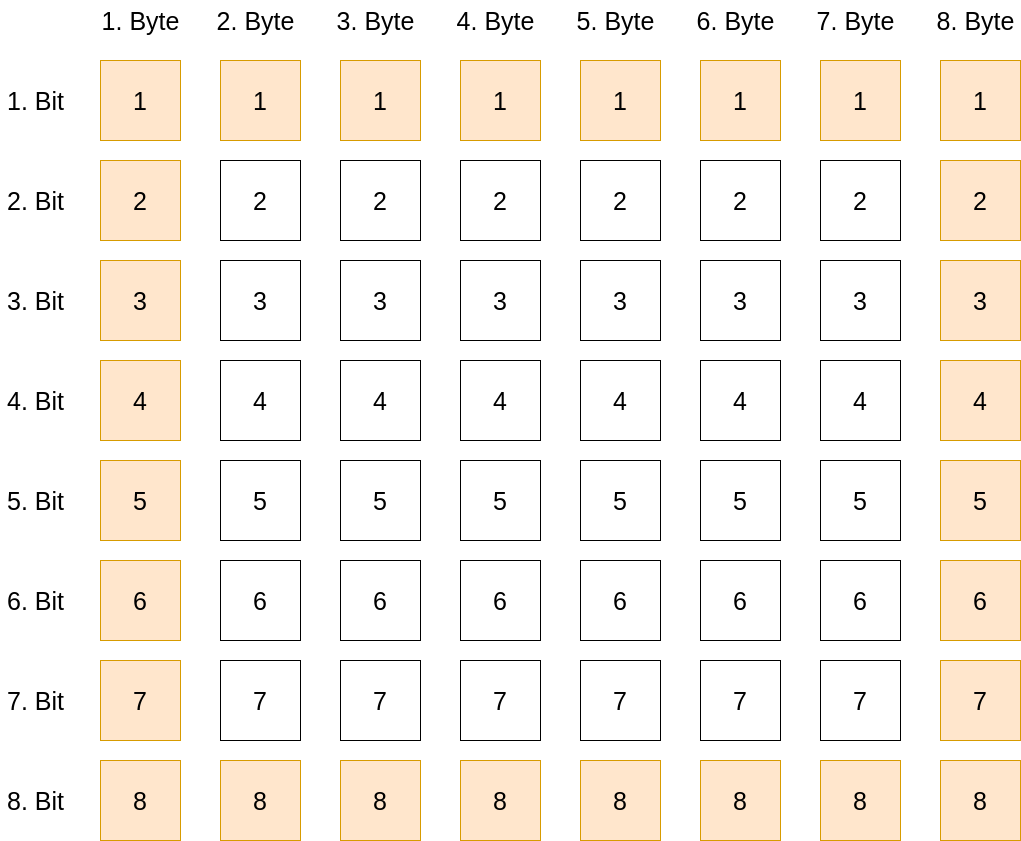
\includegraphics[scale=0.25]{img/leere-zelle.png}    
            \caption{Darstellung einer leeren Zelle im RAM}
        \end{figure}

    \subsubsection{Spieler 1 Zelle}
        Eine Zelle mit einem Spielstein von Spieler 1 ist jene, die aus Rand und aus einem gefüllten Spielstein besteht.
        \begin{figure}[H]
            \centering
            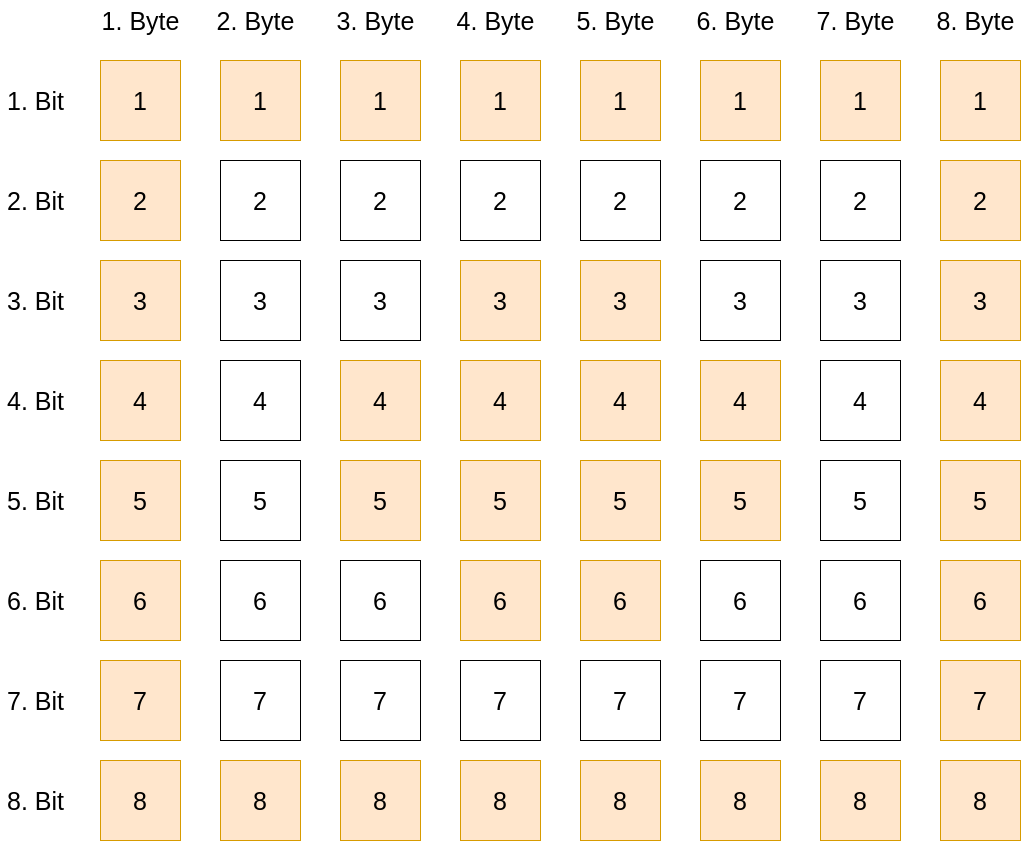
\includegraphics[scale=0.25]{img/spieler1-zelle.png}    
            \caption{Darstellung einer Zelle mit einem Spielstein von Spieler 1 im RAM}
        \end{figure}
    
    \subsubsection{Spieler 2 Zelle}
        Eine Zelle mit einem Spielstein von Spieler 1 ist jene, die aus Rand und aus einem leeren Spielstein besteht.
        \begin{figure}[H]
            \centering
            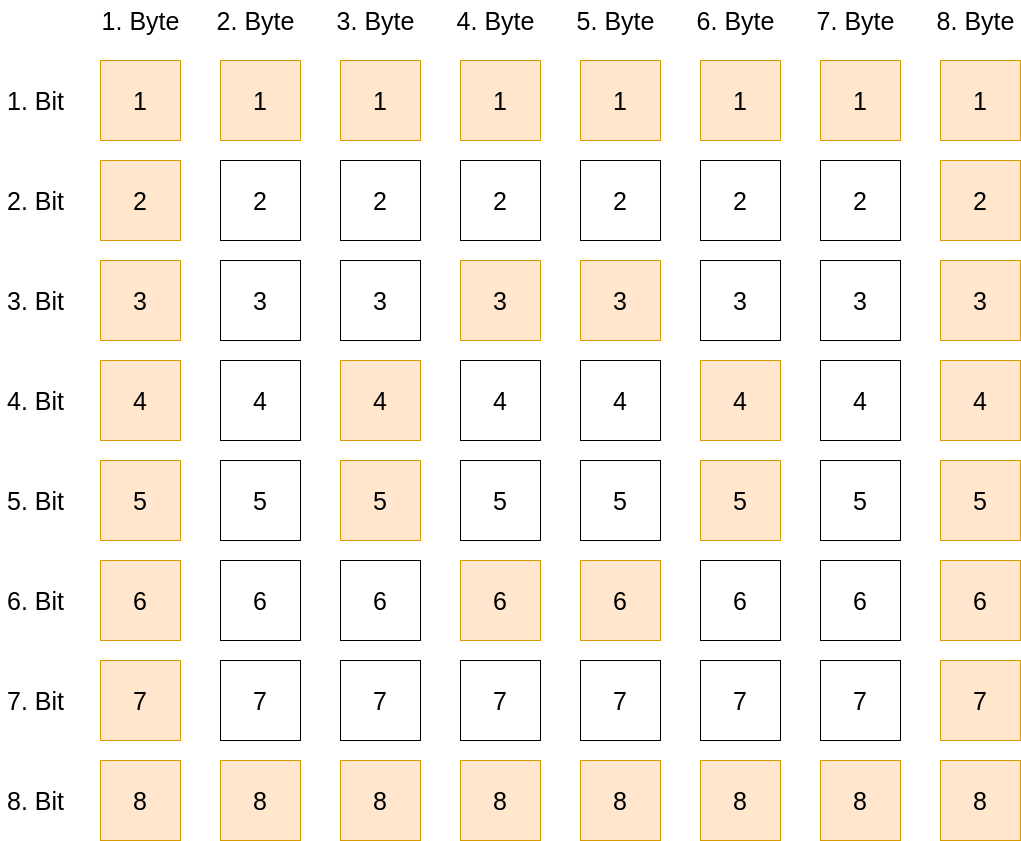
\includegraphics[scale=0.25]{img/spieler2-zelle.png}    
            \caption{Darstellung einer Zelle mit einem Spielstein von Spieler 2 im RAM}
        \end{figure}

    \subsection{Buffer}
        Das gesamte Spielfeld wird intern als Buffer repräsentiert.
        Änderungen am Spielfeld werden zunächst im Buffer getätigt, bevor der gesamte Inhalt an den LCD geschickt wird.
        \\
        Die Größe des Buffers berechnet sich dabei aus folgender Formel:
        \begin{align}
        Buffergr\ddot{o}sse = Zeilen \cdot Spalten \cdot Zellengr\ddot{o}sse
        \end{align}
        Da das Spielfeld aus sechs vertikalen Zellen und sieben horizontalen Zellen besteht und diese wiederrum aus acht Bytes bestehen,
        ergibt sich folgende Buffergröße:
        \begin{align}
        336 Byte = 6  \cdot 7  \cdot 8 Byte
        \end{align}

  





        
